\chapter[Gerenciamento do Projeto]{Gerenciamento do Projeto}

\section[Metodologia]{Metodologia}

O método que será utilizado na gestão do projeto será o Ciclo PDCA ( do inglês Plan, Do, Check, Act – Planejar, Fazer, Checar e Agir). Ele é o método gerencial mais utilizado para controle e melhoria de processos. Tal método foi desenvolvido na década de 30 pelo americano Shewhart, mas foi Deming seu maior divulgador, na década de 50. Demig ficou mundialmente conhecido ao aplicar os conceitos de qualidade no Japão. Por isso, o Ciclo PDCA também é conhecido como Ciclo de Shewhart ou, mais comumente, Ciclo de Deming \cite{pdca3}. 

Uma grande quantidade de metodologias de gestão de projetos utiliza como base o ciclo PDCA. Ao aplicá-lo de forma contínua dentro da gestão de um projeto é possível identificar erros ou falhas no desenvolvimento do projeto mais rapidamente, fazendo com que ações corretivas possam ser aplicadas tão logo quanto possível minimizando o risco de insucesso do projeto. Estar preparado para mudanças constantes e para agir rapidamente na solução de problemas em um curto espaço de tempo é útil, especialmente, para projetos que possuem curto prazo de execução, como é o caso desse projeto. 

O primeiro módulo do ciclo PDCA é o expresso pela letra P (PLANEJAR). Esse módulo é considerado como o mais importante, por ser o início do ciclo, desencadeando todo o processo referente ao ciclo PDCA. Ou seja, a eficácia futura do ciclo estará baseada em um planejamento bem elaborado e minucioso, o qual proverá dados e informações a todas as etapas restantes do método \cite{pdca1}.

Na fase do PLAN do ciclo do PDCA deve ocorrer o envolvimento de todos os integrantes da equipe, com o objetivo de procurar manter todos informados sobre as decisões do projeto, discutindo-se questões como: qual o objetivo específico (meta) a ser alcançado; quais serão os prazos e recursos necessários para realização do plano de ação; enfim, perguntas que envolvem todo um planejamento detalhado do projeto a ser executado.

A fase PLAN do ciclo PDCA, para esse projeto, foi dividida em três etapas:
\begin{enumerate}
\item Identificação do problema.
\item Estabelecimento de meta.
\item Planejamento de ação.
\end{enumerate}

A identificação do problema pode estar relacionada tanto ao problema que o produto buscará resolver quanto a problemas internos do desenvolvimento do produto, aqueles relacionados à comunicação e execução das atividades do projeto. O estabelecimento de metas refere-se ao objetivo específico que se deseja atingir em um determinado ciclo. E o planejamento de ação refere-se a planejar as atividades que serão realizadas para atingir a meta de um determinado ciclo.

A etapa posterior à etapa PLAN é definida como DO (EXECUTAR). Nesta, todas as metas e objetivos traçados na etapa anterior, e transformados em atividades ou tarefas no plano de ação, deverão ser postos em prática no prazo estabelecido pela equipe.

A etapa DO permite que o plano de ação seja praticado de forma gradual e organizado, permitindo maior eficácia das medidas a serem tomadas. A etapa de execução está voltada para a eficiência do processo produtivo \cite{pdca1}. Para que o processo seja eficiente é necessária que as atividades definidas anteriormente estejam claras para todos os integrantes da equipe e estejam bem distribuídas entre eles, também é preciso acompanhar e controlar constantemente o desenvolvimento das mesmas. 

O terceiro módulo do ciclo PDCA, CHECK (VERIFICAR) é definido como a fase de verificação das ações executadas na etapa anterior (DO). Essa fase irá se basear nos resultados das ações procedentes da fase de planejamento, e devido a esse fato, todas as ações deverão ser monitoradas adequadamente na fase EXECUTAR para que a verificação dos resultados na fase em questão possa ser realizada da maneira mais eficaz possível a fim de relatar todos os resultados obtidos com as ações pré-estipuladas \cite{pdca1}.

O último módulo do ciclo PDCA é o ACT (AGIR). Nesse projeto, esse módulo refere-se a definir as ações corretivas necessárias caso o resultado da execução das atividades não tenha atingido o objetivo definido ou relatar o que foi desenvolvido e construído caso o resultado da execução das atividades tenha atingido o objetivo definido. Se houver correções a serem feitas ou novos problemas a serem resolvidos, um novo ciclo PDCA se iniciará. 

O ciclo PDCA adaptado para o projeto está definido na figura \ref{fig03}. O ponto de parada do ciclo será quando o projeto estiver concluído ou quando o prazo do projeto estiver terminado.

\iffalse
\begin{figure}[h]
	\centering
		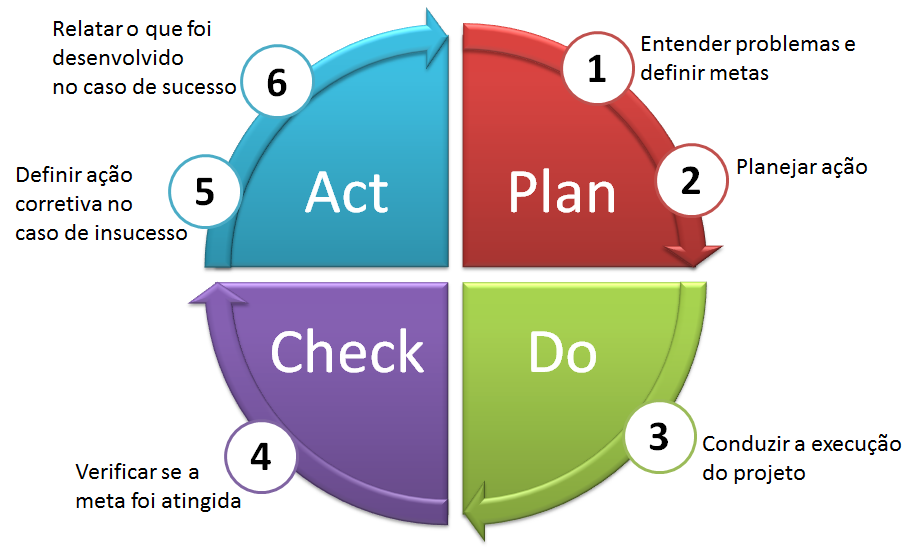
\includegraphics[keepaspectratio=true,scale=0.7]{figuras/pdca.png}
	\caption{PDCA}
	\label{fig03}
\end{figure}
\fi

\section[Recursos Humanos]{Recursos Humanos}

Os recursos humanos de um projeto são compostos pela força de trabalho humana que atuará no desenvolvimento do projeto. A equipe desse projeto contém 16 integrantes de quatro áreas de formação diferentes. As principais informações dos integrantes da equipe estão contidas na tabela 1.

\begin{table}[H]
\center
\footnotesize
\begin{tabular}{|l|l|l|l|}
\hline
\multicolumn{1}{|c}{\textbf{Nome}}  & \multicolumn{1}{|c}{\textbf{Área}}     & \multicolumn{1}{|c|}{\textbf{E-mail}} &  \multicolumn{1}{|c|}{\textbf{Telefone}}  \\ \hline
\multicolumn{1}{|c}{Aline Gonçalves}       & \multicolumn{1}{|c}{Engenharia de Software} & \multicolumn{1}{|c|}{alinegsantoss@gmail.com}               &  \multicolumn{1}{|c|}{(61)99425619}           \\ \hline
\multicolumn{1}{|c}{Beatriz Rodrigues} & \multicolumn{1}{|c}{Engenharia Eletrônica}    & \multicolumn{1}{|c|}{beatrizaraujorodrigues@gmail.com}               &\multicolumn{1}{|c|}{(61)85809701}          \\ \hline
\multicolumn{1}{|c}{Bruno Santiago}       & \multicolumn{1}{|c}{Engenharia Eletrônica}    & \multicolumn{1}{|c|}{brunosantiago\_5@hotmail.com}     & \multicolumn{1}{|c|}{(61)82573336}         \\ \hline
\multicolumn{1}{|c}{Daiane de Oliveira}   & \multicolumn{1}{|c}{Engenharia Eletrônica}                  & \multicolumn{1}{|c|}{daideoliveiradutra@hotmail.com}                & \multicolumn{1}{|c|}{(62)91902368}          \\ \hline
\multicolumn{1}{|c}{Êmille Souza} & \multicolumn{1}{|c}{Engenharia Eletrônica}     & \multicolumn{1}{|c|}{emillekessy@gmail.com}        &   \multicolumn{1}{|c|}{(61)91459364}        \\ \hline
\multicolumn{1}{|c}{Guilherme Loose}     & \multicolumn{1}{|c}{Engenharia Eletrônica}                  & \multicolumn{1}{|c|}{guilherme417@gmail.com}                & \multicolumn{1}{|c|}{(61)81276695}         \\ \hline
\multicolumn{1}{|c}{Henrique Santos}      &        \multicolumn{1}{|c}{Engenharia de Software}     &        \multicolumn{1}{|c|}{henrypsantos@hotmail.com}        & \multicolumn{1}{|c|}{(61)81090591}    \\ \hline
\multicolumn{1}{|c}{Irani Elias}                 &      \multicolumn{1}{|c}{Engenharia Eletrônica}      &            \multicolumn{1}{|c|}{irani\_jr@hotmail.com}      & \multicolumn{1}{|c|}{(62)92688937}          \\ \hline
\multicolumn{1}{|c}{Isabela Maranhão}       &   \multicolumn{1}{|c}{Engenharia de Energia}           &       \multicolumn{1}{|c|}{maranhao.bela@gmail.com}                                   & \multicolumn{1}{|c|}{(61)84494000}         \\ \hline
\multicolumn{1}{|c}{João Antonio}            &  \multicolumn{1}{|c}{Engenharia Automotiva}         &         \multicolumn{1}{|c|}{ferreira.jant@gmail.com}                                 & \multicolumn{1}{|c|}{(61)99329911}          \\ \hline
 \multicolumn{1}{|c}{Jair Junior}          &      \multicolumn{1}{|c}{Engenharia Eletrônica}         &             \multicolumn{1}{|c|}{j.junior89@hotmail.com}           & \multicolumn{1}{|c|}{(61)92262862}         \\ \hline
 \multicolumn{1}{|c}{Luciano de Paula}      &  \multicolumn{1}{|c}{Engenharia Automotiva}             &          \multicolumn{1}{|c|}{luciano.de.paula@hotmail.com}          & \multicolumn{1}{|c|}{(61)81018558}         \\ \hline
 \multicolumn{1}{|c}{Pedro Dunice}        &        \multicolumn{1}{|c}{Engenharia de Energia}       &               \multicolumn{1}{|c|}{pedro.dunice@gmail.com}                & \multicolumn{1}{|c|}{(61)82836168}          \\ \hline
 \multicolumn{1}{|c}{Raquel Melo}           &         \multicolumn{1}{|c}{Engenharia de Energia}        &              \multicolumn{1}{|c|}{limademelo.raquel@gmail.com}            & \multicolumn{1}{|c|}{(61)81238969}          \\ \hline
 \multicolumn{1}{|c}{Roberta Guimarães}         & \multicolumn{1}{|c}{Engenharia Eletrônica}     &      \multicolumn{1}{|c|}{rrosaguimaraes@gmail.com}              & \multicolumn{1}{|c|}{(61)83449232}          \\ \hline
 \multicolumn{1}{|c}{Zoé Magalhães}        &        \multicolumn{1}{|c}{Engenharia Eletrônica}                                 &             \multicolumn{1}{|c|}{zoe.roberto@hotmail.com}          & \multicolumn{1}{|c|}{(61)82379606}  \\ \hline
\end{tabular}
\caption{Recursos Humanos}
\end{table}

\subsection[Perfil da Equipe]{Perfil da Equipe}

A equipe do projeto é formada por equipes das áreas de Engenharia Automotiva, Engenharia de Energia, Engenharia de Software e Engenharia Eletrônica. A força de trabalho maior do projeto está concentrada na equipe de Engenharia de Eletrônica, no entanto, todas as equipes contêm integrantes com conhecimentos e habilidades importantes para o sucesso do projeto. O perfil da equipe do projeto é composto, portanto, pelos perfis apresentados a seguir.


\textbf{Equipe de Engenharia Automotiva}

\textbf{Conhecimentos:} Sistemas de motorização de veículos convencionais (Otto e Diesel) e alternativos, termodinâmica e fenômenos termomecânicos associados ao funcionamento veicular,
desenvolvimento de design industrial.

\textbf{Habilidades:} Ser capaz de projetar o conceito de um produto, definir mecanismos de movimento, dimensionar e realizar análise ergonômica.


\textbf{Equipe de Engenharia de Energia}

\textbf{Conhecimentos:} termodinâmica, transferência de calor, conversão eletromecânica de energia, motores, centrais de geração termoelétrica, economia da energia.

\textbf{Habilidades:} Ser capaz de definir o melhor sistema de alimentação para um produto, definir, projetar e construir sistemas que utilizam motores. 


\textbf{Equipe de Engenharia Eletrônica}

\textbf{Conhecimentos:} Desenvolvimento de circuitos eletrônicos (arquitetura de hardware), processamento de sinais, programação em microcontroladores, design de placas, desenvolvimento de sistemas embarcados, instrumentação. 

\textbf{Habilidades:} Ser capaz desenvolver e montar circuitos eletrônicos, projetar e analisar microcontroladores e microprocessadores, realizar testes, habilidades em aquisição, tratamento, análise de sinais analógicos e digitais. Programar em diversos níveis de abstração.


\textbf{Equipe de Engenharia de Software}

\textbf{Conhecimentos:} Gerenciamento de projetos, modelagem de processos, desenvolvimento de sistemas,  teste de sistemas, elicitação e análise de requisitos.

\textbf{Habilidades:} Ser capaz de adaptar-se a metodologias diversas. Atuar em todas as fases do projeto, desde o levantamento de requisitos iniciais até a construção do produto planejado. Ser capaz de acompanhar o andamento do projeto, resolver problemas, mitigar riscos e organizar a equipe. Trabalhar no desenvolvimento de relatórios e realizar pesquisas nas diversas áreas do projeto. Ser capaz de realizar estudos de viabilidade técnica e econômica, planejar e gerenciar processos e equipes de trabalho, aplicar técnicas para garantir a qualidade na produção e no software de acordo com prazos e orçamento estabelecidos

\subsection[Organograma]{Organograma}

O organograma do projeto representa graficamente os membros da equipe do projeto e suas relações hierárquicas (Fig. \ref{fig04}). Nesse projeto temos no topo da hierarquia os coordenadores das áreas de Engenharia Automotiva, Engenharia de Energia, Engenharia de Software e Engenharia Eletrônica, eles são os responsáveis pela coordenação e avaliação do projeto, auxiliados pela Estagiária Docente. A seguir está a integração das equipes das quatro áreas em uma equipe: Equipe do Posicionador de Lente, esta equipe contém líderes que se comunicarão diretamente com os coordenadores. No último nível estão as equipes das quatro áreas, que estarão trabalhando de forma auto organizadas e se comunicarão constantemente umas com as outras. 

\iffalse
\begin{figure}[h]
		\centering
			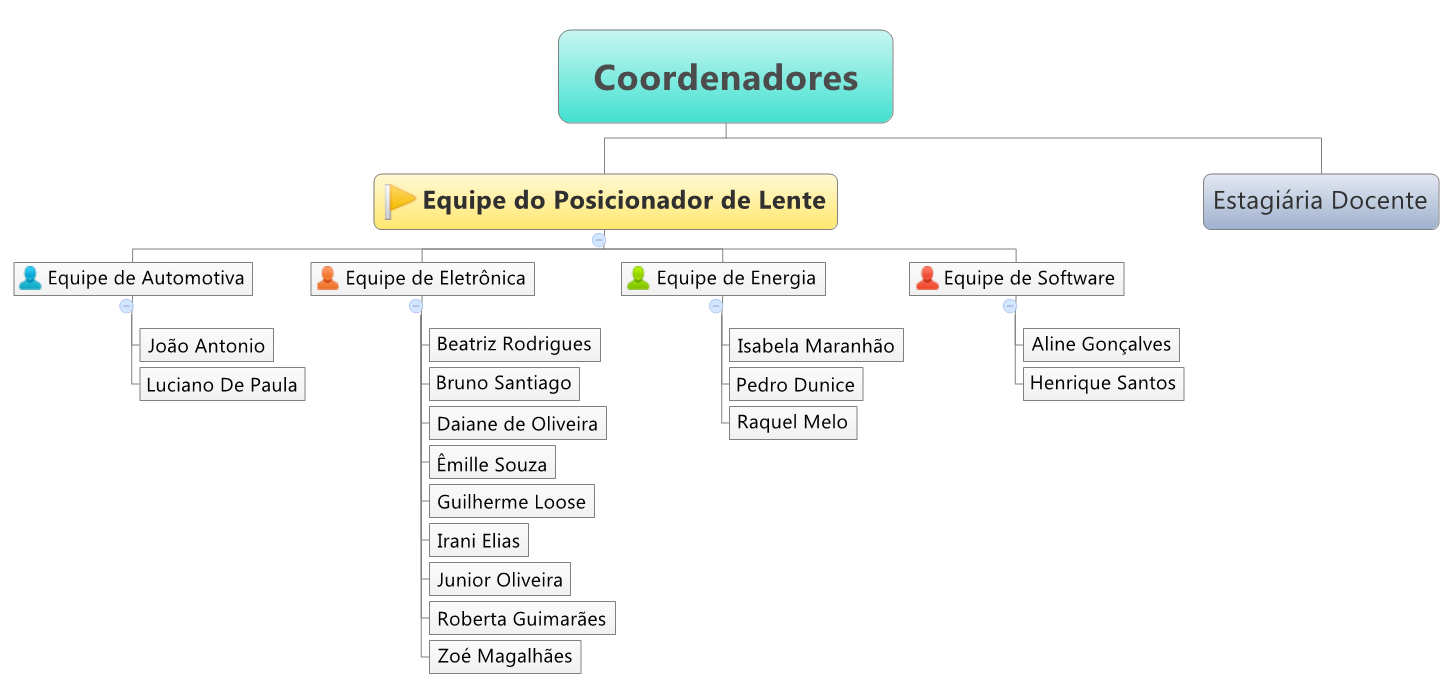
\includegraphics[scale=0.45]{figuras/organograma.png}
		\caption{Organograma}
		\label{fig04}
\end{figure}
\fi

\section[Comunicação]{Comunicação}

A comunicação eficaz entre os integrantes da equipe é primordial para o sucesso do projeto. Para tanto, é necessário definir algumas diretrizes e ferramentas que auxiliarão o processo de comunicação da equipe. São elas:

\textbf{Reuniões:}
As reuniões presenciais de cerca de 6 horas por semana serão os principais momentos de comunicação entre toda a equipe do projeto. Essas reuniões serão utilizadas para que cada subequipe relate o andamento de suas atividades para o restante do grupo, além disso, essas reuniões serão utilizadas para tomadas de decisões, divisão de próximas tarefas e construção do produto. Uma ata de reunião será feita a cada reunião e disponibilizada para toda a equipe a fim de manter todos informados sobre as principais atividades realizadas e sobre as decisões tomadas. Reuniões online poderão ser realizadas de acordo com a necessidade da equipe e com agendamento prévio. 

\textbf{Ferramentas:}

\begin{itemize}
\item Compartilhamento de Arquivos via Dropbox: ferramenta em nuvem que permite sincronizar arquivos entre os integrantes da equipe. Além disso, o Dropbox é usado como um repositório para armazenamento do que é produzido pela equipe, como documentação, código, atas de reunião, pesquisas e etc.
\item Mensagens rápidas via WhatsApp Group: ferramenta que permite a troca rápida e barata de mensagens informais entre os integrantes do grupo. Essa ferramenta será utilizada para avisos e assuntos mais urgentes.
\item Tópicos para discursão via Facebook Group ou Google Group: ferramentas que permitem discursões em tópicos de assuntos pertinentes ao projeto entre os integrantes da equipe.
\end{itemize}


\section[Recursos Materiais]{Recursos Materiais}

Para o desenvolvimento do projeto são necessários recursos materiais que serão utilizados nas diversas etapas do projeto, desde o planejamento até a construção final. Com isso, foi definida uma lista inicial dos materiais, instrumentos e ferramentas necessários para a construção do Posicionador de Lente.

\begin{itemize}	
\item Bombas
\item Cabeçote de micrômetro 
\item Câmera
\item Correia dentada
\item Cremalheira
\item Êmbolo de ferro
\item Gerador de funções 
\item Impressora 3D
\item Lentes
\item Mancal
\item Mangueiras 
\item Molas
\item Motores
\item Multímetro
\item Osciloscópio 
\item Pinça emborrachada
\item Pinhões
\item Placa de desenvolvimento micro controlada
\item Placa de desenvolvimento para sistema embarcado
\item Polia
\item Produto de limpeza de lentes
\item Rolamento
\item Sensor de distância
\item Sensor de pressão
\item Sensor de toque
\item Sensor óptico
\item Seringa de vidro
\item Software de análise estrutural
\item Software de modelagem CAD
\item Software de simulação de circuitos e layout
\item Softwares de Gestão de Projeto
\item Suporte de rosto
\item Trilho
\end{itemize}


\section[Escopo]{Escopo}

O processo de gerenciamento de escopo é definido como o trabalho que precisa ser desenvolvido para garantir a entrega de um determinado produto dentro de todas as suas especificações e funções. O escopo de um projeto pode ser dividido em três categorias: escopo funcional, escopo técnico e escopo de atividades. O escopo funcional diz respeito aos requisitos funcionais do produto, os quais serão especificados no próximo capítulo. O escopo técnico é direcionado para a equipe e consiste na definição da metodologia que será utilizada, este escopo foi definido anteriormente em Metodologia. O escopo de atividades refere-se ao trabalho a ser realizado para prover os escopos funcional e técnico do produto, este escopo estar representado graficamente na Estrutura Analítica do Projeto (Fig. \ref{fig05} e Fig. \ref{fig06}), aqual contém os pacotes de trabalho que resultaram no produto final e na documentação final do produto. 

% \begin{figure}[H]
% 		\centering
% 			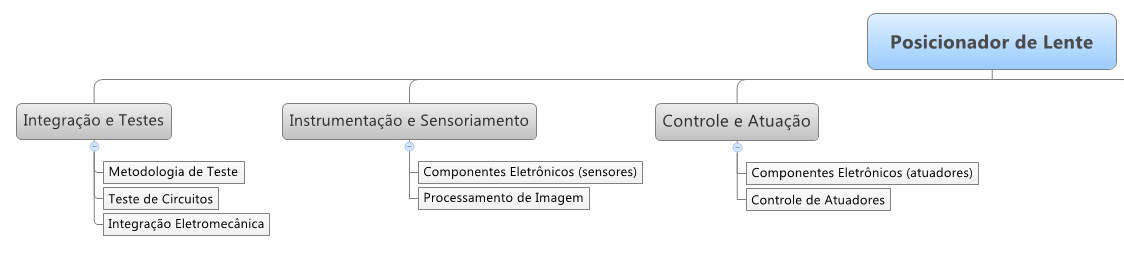
\includegraphics[scale=0.6]{figuras/eap.png}
% 		\caption{Estrutura Analítica do Projeto (EAP)}
% 		\label{fig05}
% \end{figure}


% \begin{figure}[H]
% 		\centering
% 			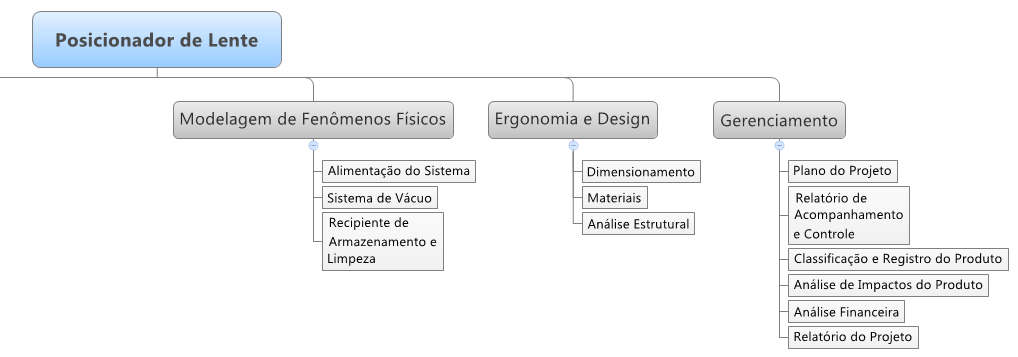
\includegraphics[scale=0.6]{figuras/eap2.png}
% 		\caption{Estrutura Analítica do Projeto (EAP) - Continuação}
% 		\label{fig06}
% \end{figure}

\section[Riscos]{Riscos}

A análise de riscos de um projeto é essencial para visualizar situações que podem colocar em risco o sucesso do projeto. Os principais tipos de riscos desse projeto são:

\begin{itemize}
\item Recursos Humanos (RH)
\item Recursos Materiais (RM)
\item Técnico (T)
\end{itemize}

Quando se pensa em riscos de Recursos Humanos é preciso pensar se existem pessoas com conhecimentos e habilidades necessárias para construir o produto. É importante voltar bastante atenção à relação recursos versus prazos, pois o risco de sobrecarga da equipe pode ocorrer. O risco de qualquer pessoa da equipe adoecer ou desistir do projeto é bastante plausível e isso causa, dependendo do papel que essa pessoa ocupava, um comprometimento no prazo e, consequentemente, no sucesso do projeto.

Os riscos de Recursos Materiais podem gerar impacto no prazo de construção do projeto. Estes riscos estão relacionados à disponibilidade dos materiais necessários para a construção do produto. Os materiais podem não ser fornecidos pela instituição de ensino, podem não estar disponíveis no mercado ou até mesmo podem ter um custo que a equipe do projeto não pode arcar. 

Os riscos técnicos giram em torno de toda parte técnica necessária para o projeto. É preciso ter conhecimento das diversas áreas que serão requeridas para construção do projeto, o que já é mitigado devido à composição multidisciplinar da equipe, porém é necessário atenção na construção do produto e prática de métodos que evitem a ocorrência de riscos dessa categoria. Estes riscos podem ocasionar diretamente o fracasso do projeto.
 
Assim, os riscos do projeto foram levantados, classificados e definidos quanto a sua severidade, também foram definidas ações de mitigação (prevenção) para esses riscos. Vale ressaltar que o próprio planejamento e gerenciamento já é uma forma de minimização de riscos. A lista de riscos está descrita na tabela 2.


\begin{table}[H]
\center
\footnotesize
\begin{tabular}{|l|l|l|l|l|l|}
\hline
\multicolumn{1}{|c|}{\textbf{ID}} & \multicolumn{1}{|c}{\textbf{Tipo}}  & \multicolumn{1}{|c}{\textbf{Risco}}  & \multicolumn{1}{|c}{\textbf{Classificação}}  & \multicolumn{1}{|c|}{\textbf{Severidade}}   \\ \hline
\multicolumn{1}{|c}{\textbf{R1}}  & \multicolumn{1}{|c}{RH} & \multicolumn{1}{|c}{Sobrecarga de determinadas pessoas da equipe}       & \multicolumn{1}{|c}{Média} & \multicolumn{1}{|c|}{Média}              \\ \hline
\multicolumn{1}{|c}{\textbf{R2}}  & \multicolumn{1}{|c}{RH} & \multicolumn{1}{|c}{Perda de integrante da equipe} & \multicolumn{1}{|c}{Baixa}    & \multicolumn{1}{|c|}{Média}             \\ \hline
\multicolumn{1}{|c}{\textbf{R3}}  & \multicolumn{1}{|c}{RM} & \multicolumn{1}{|c}{Indisponibilidade de materiais}       & \multicolumn{1}{|c}{Baixa}    & \multicolumn{1}{|c|}{Alta}          \\ \hline
\multicolumn{1}{|c}{\textbf{R4}}  & \multicolumn{1}{|c}{T} & \multicolumn{1}{|c}{Queima de componente}   & \multicolumn{1}{|c}{Baixa}                  & \multicolumn{1}{|c|}{Baixa}                      \\ \hline
\multicolumn{1}{|c}{\textbf{R5}}  & \multicolumn{1}{|c}{T} & \multicolumn{1}{|c}{Erro de Montagem} & \multicolumn{1}{|c}{Média}     & \multicolumn{1}{|c|}{Média}             \\ \hline
\multicolumn{1}{|c}{\textbf{R6}} & \multicolumn{1}{|c}{T}  & \multicolumn{1}{|c}{Erro na obtenção do sinal dos sensores}     & \multicolumn{1}{|c}{Média}                  & \multicolumn{1}{|c|}{Alta}                      \\ \hline
\multicolumn{1}{|c}{\textbf{R7}} & \multicolumn{1}{|c}{T}  & \multicolumn{1}{|c}{Erro no tratamento dos dados}      &        \multicolumn{1}{|c}{Média}     &        \multicolumn{1}{|c|}{Alta}            \\ \hline
\multicolumn{1}{|c}{\textbf{R8}} & \multicolumn{1}{|c}{T}  & \multicolumn{1}{|c}{Falha na comunicação e integração}                 &      \multicolumn{1}{|c}{Alta}      &            \multicolumn{1}{|c|}{Alta}             \\ \hline
\multicolumn{1}{|c}{\textbf{R9}} & \multicolumn{1}{|c}{T}   & \multicolumn{1}{|c}{Erro na calibração inicial}       &   \multicolumn{1}{|c}{Baixa}           &       \multicolumn{1}{|c|}{Alta}                                           \\ \hline
\multicolumn{1}{|c}{\textbf{R10}} & \multicolumn{1}{|c}{T}  & \multicolumn{1}{|c}{Erro na pressão sobre a lente}            &  \multicolumn{1}{|c}{Baixa}         &         \multicolumn{1}{|c|}{Alta}                                         \\ \hline
\multicolumn{1}{|c}{\textbf{R11}} & \multicolumn{1}{|c}{T}  &  \multicolumn{1}{|c}{Processo de limpeza da lente inadequado }          &      \multicolumn{1}{|c}{Baixa}         &             \multicolumn{1}{|c|}{Alta}               \\ \hline
\end{tabular}
\caption{Lista de Riscos}
\end{table}

As ações que a equipe de projeto irá adotar para previnir ou mitigar a ocorrência desses riscos estão descritas abaixo:

\begin{itemize}
\item \textbf{R1:}  Distribuir adequadamente as tarefas, acompanhar constantemente a execução das tarefas e integrar os módulos de forma que todos tenham conhecimento e auxiliem outros módulos do projeto quando necessário.           
\item \textbf{R2:}  Integrar os módulos de forma que todos tenham conhecimento do que está sendo feito em todas as partes do projeto.       
\item \textbf{R3:}  Buscar recursos materiais em diversos lugares (faculdade, internet, comércio).          
\item \textbf{R4:}  Adotar boas práticas de projeto.   
\item \textbf{R5:} Realizar teste de bancada.    
\item \textbf{R6:} Realizar teste de bancada.            
\item \textbf{R7:} Simular teste de bancada.   
\item \textbf{R8:} Formar equipe de teste e integração             
\item \textbf{R9:} Realizar este de bancada.  
\item \textbf{R10:} Utilizar ventosas comerciais ou especificar modelo matemático.          
\item \textbf{R11:} Projetar e Construir recipiente de armazenamento e limpeza.      
\end{itemize}

Dos riscos identificados acima, apenas o R3 ocorreu durante a execução do projeto. A impressora 3D que iria imprimir as peças do aparelho apresentou defeitos durante quatro tentativas de impressão. A ação adotada foi a definida anteriormente: buscar o recurso em diversos lugares. Com isso, buscamos uma segunda e uma terceira impressora. Porém, o prazo a essa altura para entrega do protótipo já estava acabando, com isso buscamos materiais alternativos para a construção das peças. Os principais componentes que ficaram prejudicados com essa mudança foram a caixa onde os sensores, pinça e ventosa iriam ser armazenados e a própria pinça que auxília a ventosa no processo de remoção da lente.

\section[Cronograma]{Cronograma}

O gerenciamento do tempo juntamente com o gerenciamento de custos, são as áreas mais visíveis do gerenciamento de projeto. O principal objetivo é garantir que o projeto seja concluído dentro do prazo determinado. Para tanto, é preciso definir algumas atividades e construir um cronograma exequível. Com isso, foram definidas atividades para os marcos do projeto: ponto de controle 1, ponto de controle 2 e ponto de controle 3. O Cronograma do Projeto está ilustrados na figuras \ref{fig07}, \ref{fig08} e \ref{ultimo}.

% \begin{figure}[H]
% 		\centering
% 			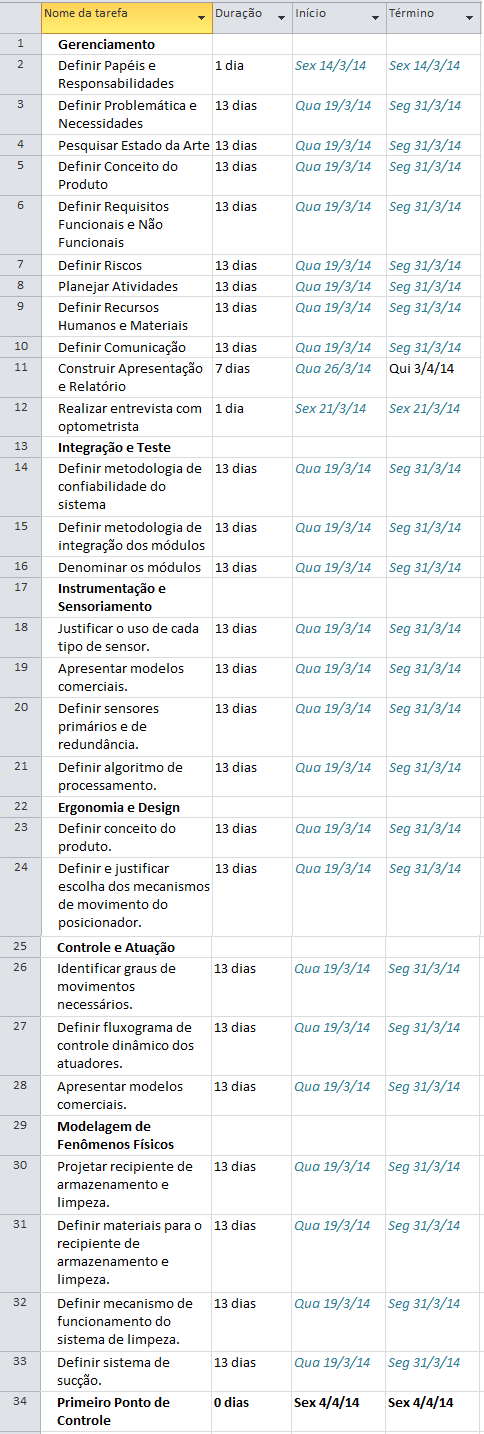
\includegraphics[scale=0.65]{figuras/cronograma1.png}
% 		\caption{Cronograma - Marco: Ponto de Controle 1}
% 		\label{fig07}
% \end{figure}


% \begin{figure}[H]
% 		\centering
% 			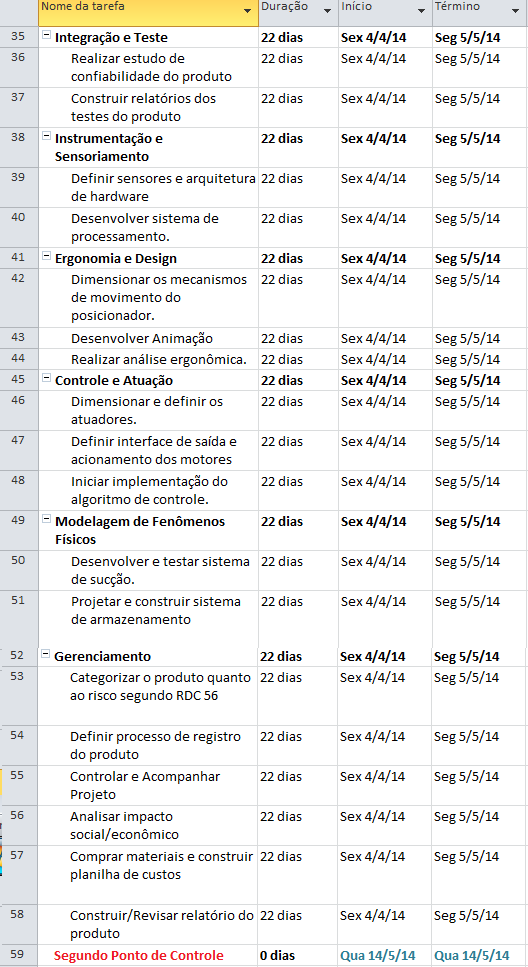
\includegraphics[scale=0.95]{figuras/cronograma2.png}
% 		\caption{Cronograma - Marco: Ponto de Controle 2}
% 		\label{fig08}
% \end{figure}

% \begin{figure}[H]
% 		\centering
% 			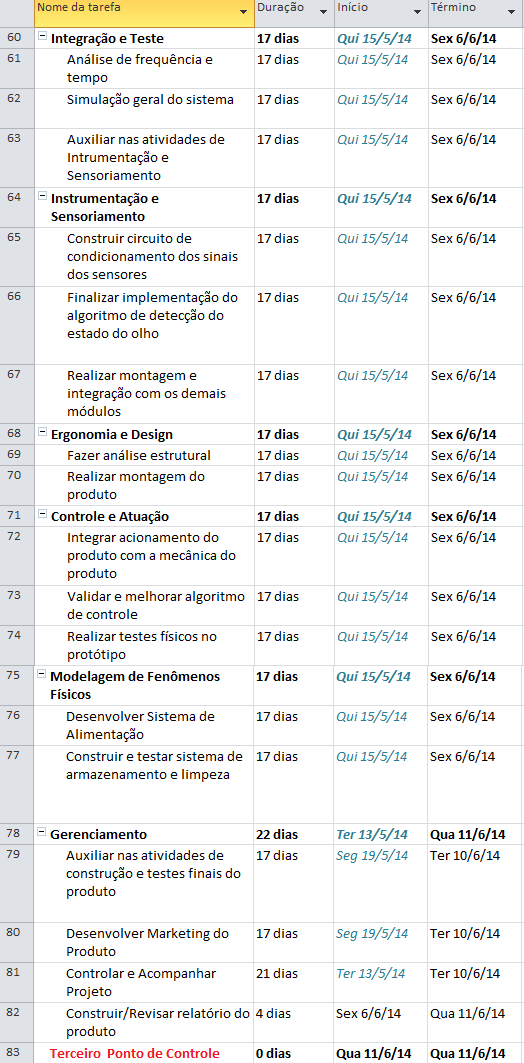
\includegraphics[scale=0.85]{figuras/cronograma3.png}
% 		\caption{Cronograma - Marco: Ponto de Controle 3}
% 		\label{ultimo}
% \end{figure}

